\documentclass[12pt,]{krantz}
\usepackage{lmodern}
\usepackage{amssymb,amsmath}
\usepackage{ifxetex,ifluatex}
\usepackage{fixltx2e} % provides \textsubscript
\ifnum 0\ifxetex 1\fi\ifluatex 1\fi=0 % if pdftex
  \usepackage[T1]{fontenc}
  \usepackage[utf8]{inputenc}
\else % if luatex or xelatex
  \ifxetex
    \usepackage{mathspec}
  \else
    \usepackage{fontspec}
  \fi
  \defaultfontfeatures{Ligatures=TeX,Scale=MatchLowercase}
    \setmonofont[Mapping=tex-ansi,Scale=0.7]{Source Code Pro}
\fi
% use upquote if available, for straight quotes in verbatim environments
\IfFileExists{upquote.sty}{\usepackage{upquote}}{}
% use microtype if available
\IfFileExists{microtype.sty}{%
\usepackage[]{microtype}
\UseMicrotypeSet[protrusion]{basicmath} % disable protrusion for tt fonts
}{}
\PassOptionsToPackage{hyphens}{url} % url is loaded by hyperref
\usepackage[unicode=true]{hyperref}
\PassOptionsToPackage{usenames,dvipsnames}{color} % color is loaded by hyperref
\hypersetup{
            pdftitle={Statistical Genetics: Analyses with R},
            pdfauthor={Dr.~Shirin Glander},
            colorlinks=true,
            linkcolor=Maroon,
            citecolor=Blue,
            urlcolor=Blue,
            breaklinks=true}
\urlstyle{same}  % don't use monospace font for urls
\usepackage{natbib}
\bibliographystyle{apalike}
\usepackage{color}
\usepackage{fancyvrb}
\newcommand{\VerbBar}{|}
\newcommand{\VERB}{\Verb[commandchars=\\\{\}]}
\DefineVerbatimEnvironment{Highlighting}{Verbatim}{commandchars=\\\{\}}
% Add ',fontsize=\small' for more characters per line
\usepackage{framed}
\definecolor{shadecolor}{RGB}{248,248,248}
\newenvironment{Shaded}{\begin{snugshade}}{\end{snugshade}}
\newcommand{\KeywordTok}[1]{\textcolor[rgb]{0.27,0.27,0.27}{\textbf{#1}}}
\newcommand{\DataTypeTok}[1]{\textcolor[rgb]{0.27,0.27,0.27}{#1}}
\newcommand{\DecValTok}[1]{\textcolor[rgb]{0.06,0.06,0.06}{#1}}
\newcommand{\BaseNTok}[1]{\textcolor[rgb]{0.06,0.06,0.06}{#1}}
\newcommand{\FloatTok}[1]{\textcolor[rgb]{0.06,0.06,0.06}{#1}}
\newcommand{\ConstantTok}[1]{\textcolor[rgb]{0,0,0}{#1}}
\newcommand{\CharTok}[1]{\textcolor[rgb]{0.5,0.5,0.5}{#1}}
\newcommand{\SpecialCharTok}[1]{\textcolor[rgb]{0,0,0}{#1}}
\newcommand{\StringTok}[1]{\textcolor[rgb]{0.5,0.5,0.5}{#1}}
\newcommand{\VerbatimStringTok}[1]{\textcolor[rgb]{0.5,0.5,0.5}{#1}}
\newcommand{\SpecialStringTok}[1]{\textcolor[rgb]{0.5,0.5,0.5}{#1}}
\newcommand{\ImportTok}[1]{#1}
\newcommand{\CommentTok}[1]{\textcolor[rgb]{0.56,0.35,0.01}{\textit{#1}}}
\newcommand{\DocumentationTok}[1]{\textcolor[rgb]{0.56,0.35,0.01}{\textbf{\textit{#1}}}}
\newcommand{\AnnotationTok}[1]{\textcolor[rgb]{0.56,0.35,0.01}{\textbf{\textit{#1}}}}
\newcommand{\CommentVarTok}[1]{\textcolor[rgb]{0.56,0.35,0.01}{\textbf{\textit{#1}}}}
\newcommand{\OtherTok}[1]{\textcolor[rgb]{0.56,0.35,0.01}{#1}}
\newcommand{\FunctionTok}[1]{\textcolor[rgb]{0.00,0.00,0.00}{#1}}
\newcommand{\VariableTok}[1]{\textcolor[rgb]{0.00,0.00,0.00}{#1}}
\newcommand{\ControlFlowTok}[1]{\textcolor[rgb]{0.13,0.29,0.53}{\textbf{#1}}}
\newcommand{\OperatorTok}[1]{\textcolor[rgb]{0.81,0.36,0.00}{\textbf{#1}}}
\newcommand{\BuiltInTok}[1]{#1}
\newcommand{\ExtensionTok}[1]{#1}
\newcommand{\PreprocessorTok}[1]{\textcolor[rgb]{0.56,0.35,0.01}{\textit{#1}}}
\newcommand{\AttributeTok}[1]{\textcolor[rgb]{0.77,0.63,0.00}{#1}}
\newcommand{\RegionMarkerTok}[1]{#1}
\newcommand{\InformationTok}[1]{\textcolor[rgb]{0.56,0.35,0.01}{\textbf{\textit{#1}}}}
\newcommand{\WarningTok}[1]{\textcolor[rgb]{0.56,0.35,0.01}{\textbf{\textit{#1}}}}
\newcommand{\AlertTok}[1]{\textcolor[rgb]{0.94,0.16,0.16}{#1}}
\newcommand{\ErrorTok}[1]{\textcolor[rgb]{0.64,0.00,0.00}{\textbf{#1}}}
\newcommand{\NormalTok}[1]{#1}
\usepackage{longtable,booktabs}
% Fix footnotes in tables (requires footnote package)
\IfFileExists{footnote.sty}{\usepackage{footnote}\makesavenoteenv{long table}}{}
\usepackage{graphicx,grffile}
\makeatletter
\def\maxwidth{\ifdim\Gin@nat@width>\linewidth\linewidth\else\Gin@nat@width\fi}
\def\maxheight{\ifdim\Gin@nat@height>\textheight\textheight\else\Gin@nat@height\fi}
\makeatother
% Scale images if necessary, so that they will not overflow the page
% margins by default, and it is still possible to overwrite the defaults
% using explicit options in \includegraphics[width, height, ...]{}
\setkeys{Gin}{width=\maxwidth,height=\maxheight,keepaspectratio}
\IfFileExists{parskip.sty}{%
\usepackage{parskip}
}{% else
\setlength{\parindent}{0pt}
\setlength{\parskip}{6pt plus 2pt minus 1pt}
}
\setlength{\emergencystretch}{3em}  % prevent overfull lines
\providecommand{\tightlist}{%
  \setlength{\itemsep}{0pt}\setlength{\parskip}{0pt}}
\setcounter{secnumdepth}{5}
% Redefines (sub)paragraphs to behave more like sections
\ifx\paragraph\undefined\else
\let\oldparagraph\paragraph
\renewcommand{\paragraph}[1]{\oldparagraph{#1}\mbox{}}
\fi
\ifx\subparagraph\undefined\else
\let\oldsubparagraph\subparagraph
\renewcommand{\subparagraph}[1]{\oldsubparagraph{#1}\mbox{}}
\fi

% set default figure placement to htbp
\makeatletter
\def\fps@figure{htbp}
\makeatother

\setmainfont[
  UprightFeatures={SmallCapsFont=AlegreyaSC-Regular}
]{Alegreya}

\renewcommand{\textfraction}{0.05}
\renewcommand{\topfraction}{0.8}
\renewcommand{\bottomfraction}{0.8}
\renewcommand{\floatpagefraction}{0.75}

\renewenvironment{quote}{\begin{VF}}{\end{VF}}

\let\oldhref\href
\renewcommand{\href}[2]{#2\footnote{\url{#1}}}

\usepackage{makeidx}\makeindex

\title{Statistical Genetics: Analyses with R}
\author{Dr.~Shirin Glander}
\date{2017-09-18}

\usepackage{amsthm}
\newtheorem{theorem}{Theorem}[chapter]
\newtheorem{lemma}{Lemma}[chapter]
\theoremstyle{definition}
\newtheorem{definition}{Definition}[chapter]
\newtheorem{corollary}{Corollary}[chapter]
\newtheorem{proposition}{Proposition}[chapter]
\theoremstyle{definition}
\newtheorem{example}{Example}[chapter]
\theoremstyle{definition}
\newtheorem{exercise}{Exercise}[chapter]
\theoremstyle{remark}
\newtheorem*{remark}{Remark}
\newtheorem*{solution}{Solution}
\let\BeginKnitrBlock\begin \let\EndKnitrBlock\end
\begin{document}
\maketitle

%\cleardoublepage\newpage\thispagestyle{empty}\null
\pagestyle{empty}\cleardoublepage\newpage

\frontmatter

{
\hypersetup{linkcolor=black}
\setcounter{tocdepth}{1}
\tableofcontents
}
\listoftables
\listoffigures
\chapter*{Preface}\label{preface}


Hi there, this is my great book.

\section*{Why read this book}\label{why-read-this-book}


It is very important\ldots{}

\section*{Structure of the book}\label{structure-of-the-book}


Chapters \ref{introduction-to-statistical-genetics} introduces a new
topic, and \ldots{}

\section*{Acknowledgments}\label{acknowledgments}


A lot of people helped me when I was writing the book.

\BeginKnitrBlock{flushright}
Shirin Glander
\EndKnitrBlock{flushright}

\chapter*{About the Author}\label{about-the-author}


I am a bioinformatician at the University Hospital of Münster in
Germany, where I'm responsible for Next Generation Sequencing analysis.
I've earned my PhD from the University of Münster, where I worked on the
link between flowering time and immune defense in plants using
quantitative genetics and RNA-sequencing. My overarching interest has
been evolutionary biology and genetics. At the moment, I am mainly
working on questions relating to immunology - specifically inflammation,
immune tolerance and auto-inflammatory diseases.

I'm a big fan of R and I write \href{www.shirin-glander.de}{a blog}
where I explore different data sets and techniques in R. I also teach
ballroom and Latin dance courses.

You can find me and my package for gene expression analysis
(exprAnalysis) on \href{https://github.com/ShirinG}{Github}.

\chapter*{The Basics of R}\label{the-basics-of-r}


\begin{quote}
``R is an integrated suite of software facilities for data manipulation,
calculation and graphical display.''
\href{https://cran.r-project.org/doc/manuals/r-release/R-intro.pdf}{An
Introduction to R - Notes on R: A Programming Environment for Data
Analysis and Graphics version 3.4.0 (2017-04-21) by W. N. Venables, D.
M. Smith and the R Core Team}
\end{quote}

R has originally been developed for statistical analysis and is a
powerful toolbox for a wide range of tasks pertaining to data handling,
statistical modeling and visualisation. It consists of a core
distribution that contains basic functions. You can use additional
packages for specific analyses.

This books assumes a basic knowledge about getting data into R,
installing and loading packages, calling functions, etc. It is beyond
the scope of this book to provide an in depth introduction to R.
Luckily, there are a large number of free online resources available,
like

\begin{itemize}
\tightlist
\item
  \href{https://cran.r-project.org/doc/manuals/r-release/R-intro.pdf}{An
  Introduction to R - Notes on R: A Programming Environment for Data
  Analysis and Graphics version 3.4.0 (2017-04-21) by W. N. Venables, D.
  M. Smith and the R Core Team}
\item
  \href{https://www.datacamp.com/courses/free-introduction-to-r}{Data
  Camp}
\item
  \href{https://onlinecourses.science.psu.edu/statprogram/r}{Penn State
  Statistics resources}
\item
  \href{http://data.princeton.edu/R/introducingR.pdf}{`Introducin R' by
  Germán Rodríguez from Princeton University}
\item
  etc.
\end{itemize}

\section*{Software information and
conventions}\label{software-information-and-conventions}


Package names are written in bold text (e.g., \textbf{rmarkdown}), and
inline code and filenames are formatted in a typewriter font (e.g.,
\texttt{plot()}). Function names are followed by parentheses (e.g.,
\texttt{bookdown::render\_book()}).

Some packages are available via
\href{https://cran.r-project.org/}{CRAN}\index{CRAN}, while others are
hosted at
\href{https://www.bioconductor.org/}{Bioconductor}\index{Bioconductor}.
I will provide package installation instructions at the beginning of
each section, indicating where each package can be found. I will also be
using the \texttt{library()} function, rather than \texttt{require()}
for loading packages to make sure that we will get an error message in
case packages have not been installed correctly.

The example workflows included are meant to illustrate the theoretical
concepts and get you started on your own analysis. They are minimal
examples of the necessary steps but are not meant to substitute the
package manuals. When you want to apply the workflows to your own data,
I highly recommend going back to the package documentation to find out
about additional functions and using the \texttt{help()} function to
explore parameter options. I will be using the same naming and code
schemes as in the package manuals to make finding the relevant parts
easy.

I used the \textbf{knitr}\index{knitr} package and the
\textbf{bookdown}\index{bookdown} package to compile this book. My R
session information is shown below:

\begin{Shaded}
\begin{Highlighting}[]
\KeywordTok{sessionInfo}\NormalTok{()}
\end{Highlighting}
\end{Shaded}

\begin{verbatim}
## R version 3.4.1 (2017-06-30)
## Platform: x86_64-apple-darwin15.6.0 (64-bit)
## Running under: macOS Sierra 10.12.6
## 
## Matrix products: default
## BLAS: /Library/Frameworks/R.framework/Versions/3.4/Resources/lib/libRblas.0.dylib
## LAPACK: /Library/Frameworks/R.framework/Versions/3.4/Resources/lib/libRlapack.dylib
## 
## locale:
## [1] de_DE.UTF-8/de_DE.UTF-8/de_DE.UTF-8/C/de_DE.UTF-8/de_DE.UTF-8
## 
## attached base packages:
## [1] stats     graphics  grDevices utils     datasets  methods   base     
## 
## loaded via a namespace (and not attached):
##  [1] compiler_3.4.1  backports_1.1.0 bookdown_0.5    magrittr_1.5   
##  [5] rprojroot_1.2   tools_3.4.1     htmltools_0.3.6 rstudioapi_0.7 
##  [9] yaml_2.1.14     Rcpp_0.12.12    stringi_1.1.5   rmarkdown_1.6  
## [13] knitr_1.17      stringr_1.2.0   digest_0.6.12   evaluate_0.10.1
\end{verbatim}

\mainmatter

\chapter{Introduction to Statistical
Genetics}\label{introduction-to-statistical-genetics}

Statistical genetics describes the scientific field that uses statistics
to gain insight from genetic data. Genetic data can help understand the
basis and regulation of traits and diseases in humans, animals, plants
and simpler organisms.

Statistical genetics makes use of large-scale datasets, e.g.~from
Genome-Wide Association Studies (GWAS) or from Next-Generation
Sequencing approaches.

\begin{itemize}
\tightlist
\item
  3rd generation of genetic markers (SNPs)
\end{itemize}

\begin{quote}
DNA sequence of numerous organisms, gene-statement information
(transcriptional profiling), and an increasing amount of knowledge about
gene function. Statisticians play an important role in the analysis and
the design of genetic studies. Statistical genetics overlaps with fields
such as biomathematics, bioinformatics, biology, epidemiology, genetics,
etc. People in the department have worked and are working on methods in
linkage analysis, allelic association tests, gene statement array data
analysis, sequence analysis, comparative genomics, phylogenetic tree
reconstruction, etc.
\end{quote}

Statistical inference of genetic regulation needs sufficiently large
study populations, especially if we analyse unrelated individuals.
Family cohort analyses can be done on much smaller sample sizes, because
we can largely assume Mendelian inheritance.

A solid understanding of inheritance mechanisms in populations is
paramount to understanding statistical genetics. Therefore, this book
will start with evolutionary and population genetics, the subfield that
studies evolutionary processes like speciation and adaptation or
population-level phenomena like migration, drift, etc.

Closely related to population genetics is quantitative genetics. Here,
the focus lies on analysing quantitative traits and their underlying
genetic regulation.

\begin{quote}
Genetic epidemiology is the study of the role of genetic factors in
determining health and disease in families and in populations, and the
interplay of such genetic factors with environmental factors. Genetic
epidemiology seeks to derive a statistical and quantitative analysis of
how genetics work in large groups.{[}1{]}
\end{quote}

\begin{quote}
Statistical genetics is concerned with the analysis of genetic data. Due
to rapid progress in laboratory techniques, there is an ever-increasing
slew of new data: the 3rd generation of genetic markers (SNPs), the DNA
sequence of numerous organisms, gene-statement information
(transcriptional profiling), and an increasing amount of knowledge about
gene function. Statisticians play an important role in the analysis and
the design of genetic studies. Statistical genetics overlaps with fields
such as biomathematics, bioinformatics, biology, epidemiology, genetics,
etc. People in the department have worked and are working on methods in
linkage analysis, allelic association tests, gene statement array data
analysis, sequence analysis, comparative genomics, phylogenetic tree
reconstruction, etc.
\end{quote}

\begin{quote}
Statistical geneticists at HSPH develop statistical methods for
understanding the genetic basis of human diseases and traits. These
methods involve large-scale data sets from candidate-gene, genome-wide
and resequencing studies, using both unrelated and related individuals.
HSPH statistical geneticists collaborate with other investigators at
HSPH and around the world on studies of cancer, heart disease, diabetes,
respiratory disease, psychiatric disease, and health-related behaviors
(e.g.~smoking, diet). They have close ties to the Program in
Quantitative Genomics and Computational Biology and Bioinformatics group
at HSPH. Training encompasses basic statistics; Mendelian and population
genetics; design and analysis of genetic association studies; gene
expression and epigenetic markers; and gene-environment interaction.
\end{quote}

\begin{quote}
The human genome project is changing the practice of medicine and public
health, and genetics is playing an ever more central role in all the
biomedical sciences. This expanding role includes the mapping and
sequencing of the human genome and the genomes of other organisms, the
identification of all human genes and the cataloging of all common human
genetic variants, the development of methods to assay the expression of
many genes simultaneously, the investigation of the molecular evolution
of human genes, and the translation of the resulting knowledge to
address questions of human health and disease. These developments
present remarkable opportunities for the prevention and cure of human
disease, but require investigators working at the interface between
human genetics and the mathematical sciences
\end{quote}

\url{https://cran.r-project.org/web/views/Genetics.html}
\url{https://www.mcgill.ca/statisticalgenetics/software}

\chapter{Evolutionary and Population
Genetics}\label{evolutionary-and-population-genetics}

Evolutionary and population genetics study processes like adapation and
speciation events from a genetic perspective. This means that they are
interested in how genes and alleles are transmitted between parents and
offspring (or in some cases even horizontally), how they change and
adapt over time , how dominance, epistasis and epigenetics influence
phenotypes and how this relate to population structure.

The basic concept of evolutionary biology is that in order for selection
to lead to change in populations, there needs to be sufficient genetic
and phenotypic variation in that population to select from. From a
genetics perspective, this means that selection will favor certain
alleles among the pool of genes in the population. Favorable alleles
will therefore increase in frequency within the population over time,
while disadvantageous alleles will eventually disappear. Depending on
how stable the environment is, this change in allele frequencies can be
subject to severe fluctuation.

Additional aspects like migration, mutation, recombination, inbreeding,
drift, etc. make modeling of evolutionary and population genetic
processes non-trivial.

\url{https://en.wikipedia.org/wiki/Population_genetics}

\begin{itemize}
\tightlist
\item
  Mendelian and population genetics;
\end{itemize}

\section{Evolution of Genetic
Systems}\label{evolution-of-genetic-systems}

\section{Phylogenetics}\label{phylogenetics}

\section{Game Theory}\label{game-theory}

\section{Genetic Algorithms}\label{genetic-algorithms}

\section{Evolutionary Algorithms}\label{evolutionary-algorithms}

\section{Hardy-Weinberg}\label{hardy-weinberg}

\section{Linkage Disequilibrium}\label{linkage-disequilibrium}

\chapter{Quantitative Genetics}\label{quantitative-genetics}

\begin{itemize}
\item
  gene expression and epigenetic markers
\item
  gene-environment interaction
\end{itemize}

\url{http://nitro.biosci.arizona.edu/zbook/book.html}

\section{QTL analysis}\label{qtl-analysis}

Quantitative Trait Loci (QTL) are regions in the genome that are
associated with variation in a quantitative trait. Quantitative traits
are phentoypes that can be measured on a continuous scale, like height,
weight, etc.

QTL analysis (or QTL mapping) is typically done on experimental
populations to find genes which contribute to the heritability of
traits. Phenotype and genetic marker data are collected from every
individual in the population. The general concept of QTL mapping is that
we can then calculate the correlation between genotypes and phenotypes
at each marker position and test whether they show a statistically
significant association.

Let's consider the famous example of \citet{Doebley285}, who assessed
the variation of traits that discriminate commercial maize from its
native relative teosinte. Teosinte is much smaller than maize as we know
it today and one teosinte plant produces many ears, each of which has
only two rows of seeds. But even though maize and teosinte look so
completely different, they are still able to produce viable offspring
together. \citet{Doebley285} utilized this and crossed the two plant
species to produce an F1 generation, which were in turn self-pollinated.
The resulting F2 population of maize-teosinte-hybrids showed a wide
range of intermediate parental morphologies. Each of the F2 offspring
was then genotyped at 58 locations in the genome, so that the
quantitative trait information on morphology could be correlated with
the genetic map. This analysis revealed that most of the morphological
variation between maize and teosinte were the result of changes in only
a handful of genes, one of which is the \emph{tb1} (\emph{teosinte
branched 1}) gene.

\subsection{Recombinant Inbred Lines
(RILs)}\label{recombinant-inbred-lines-rils}

RILs are experimental sister populations that have been produced by a
very specific back-crossing scheme. The process is similar to Doebley
and Stec's crossing of maize and teosinte: two homozygous parents are
crossed to produce an F1 generation. Following the laws of genetics,
each offspring's genome consists of a random combination of parental
alleles and crossover (or recombination) events. Depending on the
design, F1 offspring are usually either selfed or mated with a sibling
to introduce another level of genetic recombination. The final
generation is then inbred for many generations to obtain a collection of
homozygous sister lines, each with a unique mosaic genome of parental
alleles \citep{Pollard2012}.

\subsection{QTL analysis in R}\label{qtl-analysis-in-r}

\subsubsection{The qtl package}\label{the-qtl-package}

The most established R package for QTL mapping is Karl Broman's
\href{http://www.rqtl.org/}{\textbf{qtl} package}\index{qtl}
\citep{R-qtl}. It implements several techniques for finding QTLs, like
Hidden Markov Models (HMM), interval mapping, Haley-Knott regression and
multiple imputation. It is very well documented and comes with extensive
example data and code.

Here, I will introduce you to a basic QTL mapping workflow using the
examples given in the package documentation and refer you to more
complex analysis options where applicable.

\paragraph{Installation and loading the
package}\label{installation-and-loading-the-package}

If this is the first time you are using the \textbf{qtl}\index{qtl}
package, you need to install it from CRAN. The following line of code
checks whether you already have the package, and if not installs it.

\begin{Shaded}
\begin{Highlighting}[]
\NormalTok{pkg =}\StringTok{ "qtl"}
\ControlFlowTok{if}\NormalTok{ (}\KeywordTok{system.file}\NormalTok{(}\DataTypeTok{package =}\NormalTok{ pkg) }\OperatorTok{==}\StringTok{ ''}\NormalTok{) }\KeywordTok{install.packages}\NormalTok{(pkg)}
\end{Highlighting}
\end{Shaded}

You can then load the package:

\begin{Shaded}
\begin{Highlighting}[]
\KeywordTok{library}\NormalTok{(qtl)}
\end{Highlighting}
\end{Shaded}

\paragraph{Loading the data}\label{loading-the-data}

I will be using the example data on murine hypertension that is provided
in the package \citep{Sugiyama200170}. In this dataset, we find
information on 250 male mice from a reciprocal backcross between two
strains: 1) the salt-sensitive C57BL/6J strain or 2) the inbred
normotensive A/J strain. These mice were then given 1\% salt water over
two weeks and their hypertension blood pressure levels were measured.

\begin{Shaded}
\begin{Highlighting}[]
\KeywordTok{data}\NormalTok{(hyper)}
\end{Highlighting}
\end{Shaded}

It is - as always - a good idea to familiarize yourself with the data to
identify potential problems or errors before spending hours or days on
an analysis that leads nowhere. The \texttt{summary()} function shows
you the main properties of the data, like number of individuals and
phenotypes, genotype information and proportion of missing data.

\begin{Shaded}
\begin{Highlighting}[]
\KeywordTok{summary}\NormalTok{(hyper)}
\end{Highlighting}
\end{Shaded}

\begin{verbatim}
##     Backcross
## 
##     No. individuals:    250 
## 
##     No. phenotypes:     2 
##     Percent phenotyped: 100 100 
## 
##     No. chromosomes:    20 
##         Autosomes:      1 2 3 4 5 6 7 8 9 10 11 12 13 14 15 16 17 18 19 
##         X chr:          X 
## 
##     Total markers:      174 
##     No. markers:        22 8 6 20 14 11 7 6 5 5 14 5 5 5 11 6 12 4 4 4 
##     Percent genotyped:  47.7 
##     Genotypes (%):    
##           Autosomes:    BB:50.1  BA:49.9 
##        X chromosome:    BY:53.0  AY:47.0
\end{verbatim}

\begin{Shaded}
\begin{Highlighting}[]
\KeywordTok{plot}\NormalTok{(hyper)}
\end{Highlighting}
\end{Shaded}

\begin{figure}
\centering
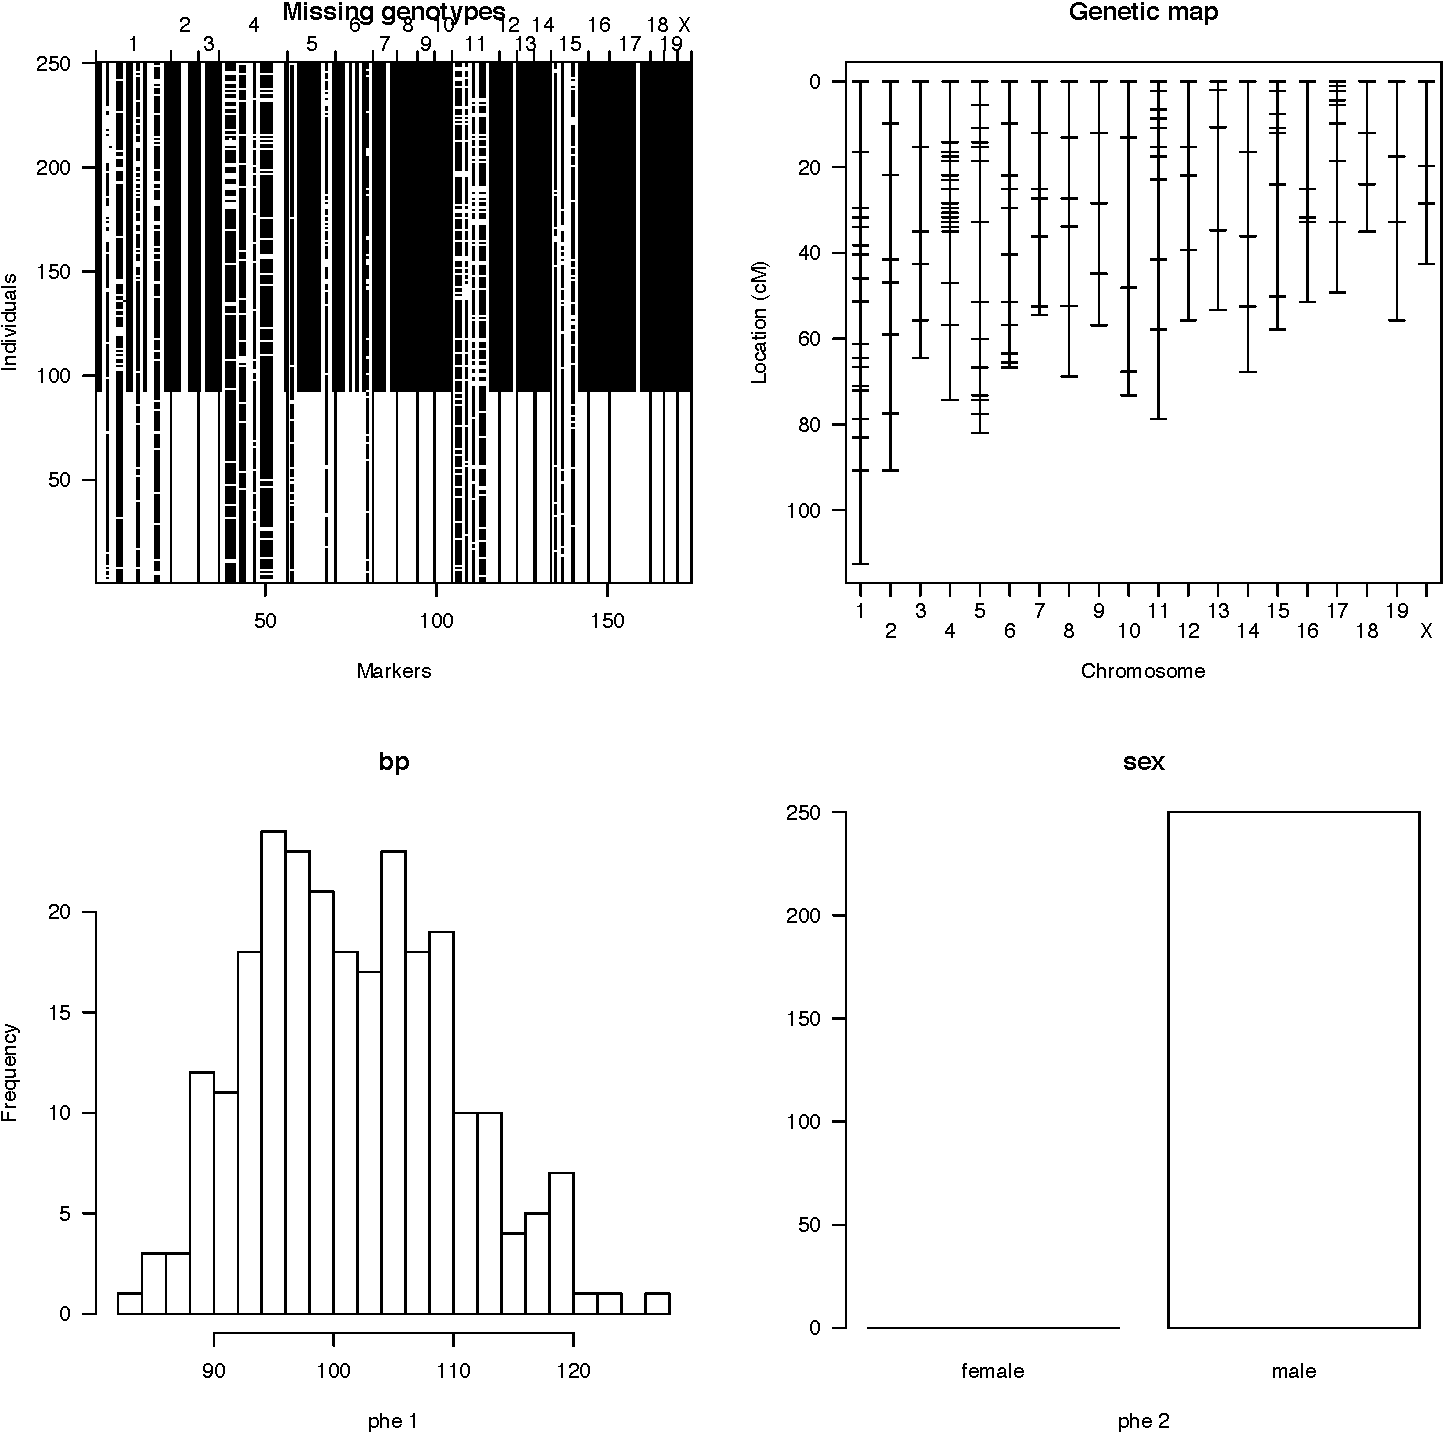
\includegraphics{_main_files/figure-latex/qtl-plot-hyper-1.pdf}
\caption{\label{fig:qtl-plot-hyper}Plots providing an overview over missing
genotypes, marker positions and the distribution of phenotypes or
traits. Plots were generated with \texttt{qtl::plot()}. In the upper
left plot markers are shown against individuals, with black areas
showing missing information. As we can see here, there is quite a bit of
missing data. The upper right plot shows the marker positions on the
chromosomes. Here, we can easily see that chromosomes 1, 4, 11 and 17
have clusters of more densely positioned markers. The lower plots show
phenotype information, either as a histogram for continuous values or as
a bar chart for categorical factors.}
\end{figure}

The \texttt{plot()} function produces plots that show missing genotypes,
marker positions and the distribution of phenotypes or traits. Figure
\ref{fig:qtl-plot-hyper} will give you a first idea about the quality of
your data.

The \href{http://www.rqtl.org/tutorials/rqtltour.pdf}{package manual}
includes a description of various additional plotting functions, which I
won't cover here.

\paragraph{Genetic map estimation}\label{genetic-map-estimation}

Before we proceed with the analysis, I typically recommend replacing the
existing genetic map with an estimated one to reduce the potential
errors. The genetic map represents all markers on a chromosome in a
linear fashion. The `est.map() function applies a Hidden Markov Model
\citep{Lander01041987} to estimate the map with an assumed genotyping
error rate (\emph{error.prob}).

Here, we can also specify the mapping function (\emph{map.function})
that we want to use to convert genetic distance to recombination
fraction. The distance between two markers is usually given as a unit of
genetic linkage, called \emph{centimorgan (cM)} One cM represents the
distance with an average of 0.01 crossover events in one generation
(i.e.~1\% recombination). However, this representation of distance
underestimates the actual recombination fraction, which is inherently
not additive. With increasing distance the chance of double crossovers
increases, so that they are in a way ``invisible'' to the traditional
estimation of recombination distance.

Another reason why genetic maps based on recombination are biased is
crossover interference, which described the phenomenon that a crossover
event reduces the likelihood of another recombination event occur close
by.

To correct for such biases, we can choose from the following mapping
functions:

\begin{itemize}
\tightlist
\item
  \textbf{Haldane's} is the simplest mapping function and assumes a
  Poisson distribution for crossover events and does not consider
  interference.
\item
  \textbf{Kosambi's} mapping function also considers interference and
  double crossovers but it can not calculate joint recombination
  probabilities for more than three loci.
\item
  \textbf{Carter-Falconer's} mapping function can be extended to more
  complex interference rates.
\item
  \textbf{Morgan's} mapping function assumes complete interference.
\end{itemize}

The two most widely used mapping functions are Haldane's (the default)
and Kosambi's. For this example, using Haldane's should be sufficient.
Because our example is a backcross, we can assume no interference,
meaning that all crossovers are independent \citep{lynch1998genetics}.

\begin{Shaded}
\begin{Highlighting}[]
\NormalTok{newmap <-}\StringTok{ }\KeywordTok{est.map}\NormalTok{(hyper, }\DataTypeTok{error.prob =} \FloatTok{0.0001}\NormalTok{, }
                  \DataTypeTok{map.function =} \StringTok{"haldane"}\NormalTok{)}
\NormalTok{hyper <-}\StringTok{ }\KeywordTok{replace.map}\NormalTok{(hyper, newmap)}
\end{Highlighting}
\end{Shaded}

We can now estimate the recombination fractions between all pairs of
markers. The \texttt{est.rf()} function also calculates the LOD scores.
LOD stands for ``likelihood of the odds'' and is a measure of linkage.
In QTL mapping we calculate LOD scores for the genetic markers and a
threshold, above which we consider a QTL statistically significant in
its association with the trait.

\begin{Shaded}
\begin{Highlighting}[]
\NormalTok{hyper <-}\StringTok{ }\KeywordTok{est.rf}\NormalTok{(hyper)}
\end{Highlighting}
\end{Shaded}

The \texttt{calc.errorlod()} function calculates the genotyping errors
according to \citet{Lincoln1992604}. We can see which markers have an
error LOD above a certain threshold (cutoff) with the
\texttt{top.errorlod()} function (Table \ref{tab:qtl-te}).

\begin{Shaded}
\begin{Highlighting}[]
\NormalTok{hyper <-}\StringTok{ }\KeywordTok{calc.errorlod}\NormalTok{(hyper, }\DataTypeTok{error.prob =} \FloatTok{0.0001}\NormalTok{)}
\NormalTok{te <-}\StringTok{ }\KeywordTok{top.errorlod}\NormalTok{(hyper, }\DataTypeTok{cutoff =} \DecValTok{3}\NormalTok{)}
\end{Highlighting}
\end{Shaded}

\begin{longtable}[]{@{}lrlr@{}}
\caption{\label{tab:qtl-te}Markers with an error LOD bigger than 3 under an
error probability of 0.0001 indicate potential genotyping
errors.}\tabularnewline
\toprule
chr & id & marker & errorlod\tabularnewline
\midrule
\endfirsthead
\toprule
chr & id & marker & errorlod\tabularnewline
\midrule
\endhead
4 & 102 & D4Mit288 & 3.324582\tabularnewline
4 & 107 & D4Mit111 & 3.262205\tabularnewline
4 & 216 & D4Mit214 & 3.261092\tabularnewline
11 & 57 & D11Mit82 & 3.021105\tabularnewline
11 & 118 & D11Mit82 & 3.021105\tabularnewline
\bottomrule
\end{longtable}

These potentially erroneous markers can then be removed or set to
\texttt{NA}.

\begin{Shaded}
\begin{Highlighting}[]
\NormalTok{hyper.clean <-}\StringTok{ }\NormalTok{hyper}
\ControlFlowTok{for}\NormalTok{ (i }\ControlFlowTok{in} \DecValTok{1}\OperatorTok{:}\KeywordTok{nrow}\NormalTok{(te)) \{}
\NormalTok{  chr <-}\StringTok{ }\NormalTok{te}\OperatorTok{$}\NormalTok{chr[i]}
\NormalTok{  id <-}\StringTok{ }\NormalTok{te}\OperatorTok{$}\NormalTok{id[i]}
\NormalTok{  mar <-}\StringTok{ }\NormalTok{te}\OperatorTok{$}\NormalTok{marker[i]}
\NormalTok{  hyper.clean}\OperatorTok{$}\NormalTok{geno[[chr]]}\OperatorTok{$}\NormalTok{data[hyper}\OperatorTok{$}\NormalTok{pheno}\OperatorTok{$}\NormalTok{id }\OperatorTok{==}\StringTok{ }\NormalTok{id, mar] <-}\StringTok{ }\OtherTok{NA}
\NormalTok{\}}
\end{Highlighting}
\end{Shaded}

\paragraph{Finding QTLs}\label{finding-qtls}

Now, we can proceed with the central step: mapping the QTLs.

Because the individuals in QTL studies are genotyped at specific marker
locations throughout the genome, we inherently have to deal with the
missing information about genotypes between markers. Hidden Markov
Models (HMM) can help us overcome this problem by calculating genotype
probabilities between markers based on the joint genotype distribution.

We first need to calculate these genotype probabilities using the
\texttt{calc.genoprob()} function. We can define several parameters,
like step size, the amount of error we want to allow for, the mapping
function and step width. Here, we want to calculate genotype
probabilities for every cM (step = 1), with a fixed step width and an
error probability of 0.0001. As above, we are again using Haldane's
mapping function.

\begin{Shaded}
\begin{Highlighting}[]
\NormalTok{hyper.clean <-}\StringTok{ }\KeywordTok{calc.genoprob}\NormalTok{(hyper.clean, }\DataTypeTok{step =} \DecValTok{1}\NormalTok{, }
                             \DataTypeTok{error.prob =} \FloatTok{0.0001}\NormalTok{, }
                             \DataTypeTok{map.function =} \StringTok{"haldane"}\NormalTok{, }
                             \DataTypeTok{stepwidth =} \StringTok{"fixed"}\NormalTok{)}
\end{Highlighting}
\end{Shaded}

The simplest QTL model, we can run is single-QTL marker regression or
interval mapping using the \texttt{scanone()} function.

These simple methods can give a good estimation of QTLs but they can
also introduce bias, especially with multiple QTL in close proximity.
More advanced mapping approaches, like Composite Interval Mapping (CIM)
are discussed later on.

The first parameter we want to specify is the phenotype(s) and model
(e.g.~parametric or non-parametric) for mapping. Here, we want to use
the first phenotype, i.e.~the first column in our phenotype matrix,
which follows a normal distribution. We can see the phenotype matrix by
calling:

\begin{Shaded}
\begin{Highlighting}[]
\NormalTok{hyper.clean}\OperatorTok{$}\NormalTok{pheno}
\end{Highlighting}
\end{Shaded}

Then, we need to specify the mapping algorithm we want to use. We can
choose from several options. Here, I will only present the practical
implications for each method. For a full discussion of the mathematical
principles, see \citet{lynch1998genetics}.

\begin{itemize}
\tightlist
\item
  \textbf{Marker regression}: Marker regression is by far the simplest
  approach to QTL mapping. Here, we calculate the association between
  phenotype and genotype at each marker position independently.
\end{itemize}

Because it is so simple, marker regression is seldom recommended to use.
With interval mapping, a phenotype \textasciitilde{} genotype
association analysis is performed for each flanking marker pair
independently. This improves the approximation and gives confidence
regions around QTL.

\begin{itemize}
\tightlist
\item
  \textbf{EM (Expectation-Maximization) algorithm}: EM is usually
  applied to maximum likelihood (ML) analyses of mixed models. It is an
  iterative process of calculating conditional probabilities and
  updating the ML estimates. This process is repeated until the
  estimates converge \citep{Lander185}. If we have a reasonably dense
  marker map, the EM algorithm will converge on the global maximum.
\item
  \textbf{(Extended) Haley-Knott regression}: Haley-Knott regression
  uses a simpler model than the EM algorithm \citep{Haley1992}. The
  extended Haley-Knott regression also considers variance is therefore
  gives improved approximations. Haley-Knott regression can give good
  approximations of the likelihood profiles for ML interval mapping but
  with more complex cases, it can be heavily biased.
\item
  \textbf{Multiple imputation}: This method uses multiple rounds of
  imputing the unknown genotypes between markers and combines them into
  a final imputation model \citep{Sen371}. This allows us to perform a
  simple analysis of variance at each position in the genome. Multiple
  imputation needs much more computational power than simpler methods
  and will usually not outperform them with single-QTL models (it is
  much more advantageous with more complex multi-QTL models, however).
\end{itemize}

Here, I will show QTL mapping examples for the EM algorithm and for
multiple imputation:

\begin{Shaded}
\begin{Highlighting}[]
\CommentTok{# EM algorithm}
\NormalTok{out.em <-}\StringTok{ }\KeywordTok{scanone}\NormalTok{(hyper.clean, }\DataTypeTok{pheno.col =} \DecValTok{1}\NormalTok{, }\DataTypeTok{model =} \StringTok{"normal"}\NormalTok{, }
                  \DataTypeTok{method =} \StringTok{"em"}\NormalTok{)}
\end{Highlighting}
\end{Shaded}

The multiple imputation method requires the use of the
\texttt{sim.geno()} function before we call the mapping function. It
calculates the joint genotype distribution based on the available marker
information and uses it to perform the imputation of missin genotypes.
With the \texttt{n.draws} parameter, we define how many imputations will
be run. The more imputations steps we run, the more precise the
genotypes but with increasing cost of computational time and power.

\begin{Shaded}
\begin{Highlighting}[]
\NormalTok{hyper.clean <-}\StringTok{ }\KeywordTok{sim.geno}\NormalTok{(hyper.clean, }\DataTypeTok{step =} \DecValTok{1}\NormalTok{, }\DataTypeTok{n.draws =} \DecValTok{100}\NormalTok{, }
                        \DataTypeTok{error.prob =} \FloatTok{0.0001}\NormalTok{, }
                        \DataTypeTok{map.function =} \StringTok{"haldane"}\NormalTok{, }
                        \DataTypeTok{stepwidth =} \StringTok{"fixed"}\NormalTok{)}

\NormalTok{out.imp <-}\StringTok{ }\KeywordTok{scanone}\NormalTok{(hyper.clean, }\DataTypeTok{pheno.col =} \DecValTok{1}\NormalTok{, }\DataTypeTok{model =} \StringTok{"normal"}\NormalTok{, }
                   \DataTypeTok{method =} \StringTok{"imp"}\NormalTok{)}
\end{Highlighting}
\end{Shaded}

Now that we have a LOD score for each marker position, we want to know
which positions are significantly associated with the phenotype. To
determine this, we will use the \textbf{scanone()} function again, but
this time we want to calculate the genome-wide LOD score threshold with
a permutation test. Above this threshold we can consider a QTL to be
statistically significant. Here, I am using a similar call as before,
but I am specifying that we want to use 1000 permutations.

\begin{Shaded}
\begin{Highlighting}[]
\NormalTok{operm.imp <-}\StringTok{ }\KeywordTok{scanone}\NormalTok{(hyper.clean, }\DataTypeTok{pheno.col =} \DecValTok{1}\NormalTok{, }\DataTypeTok{model =} \StringTok{"normal"}\NormalTok{, }
                     \DataTypeTok{method =} \StringTok{"imp"}\NormalTok{, }\DataTypeTok{n.perm =} \DecValTok{1000}\NormalTok{)}
\end{Highlighting}
\end{Shaded}

The \texttt{summary()} function will tell us our genome-wide LOD score
threshold for a given significance value (here 0.05).

\begin{Shaded}
\begin{Highlighting}[]
\NormalTok{lod <-}\StringTok{ }\KeywordTok{summary}\NormalTok{(operm.imp, }\DataTypeTok{alpha =} \FloatTok{0.05}\NormalTok{)}
\NormalTok{lod}
\end{Highlighting}
\end{Shaded}

\begin{verbatim}
## LOD thresholds (1000 permutations)
##     lod
## 5% 2.34
\end{verbatim}

And now we can also refine our QTL results by including the significance
threshold. This will give us the LOD score and estimated p-values for
each marker above the threshold, around which we can now assume to have
found a QTL for our trait of interest.

\begin{Shaded}
\begin{Highlighting}[]
\KeywordTok{summary}\NormalTok{(out.imp, }\DataTypeTok{perms =}\NormalTok{ operm.imp, }\DataTypeTok{alpha =} \FloatTok{0.05}\NormalTok{, }\DataTypeTok{pvalues =} \OtherTok{TRUE}\NormalTok{)}
\end{Highlighting}
\end{Shaded}

\begin{verbatim}
##           chr   pos  lod  pval
## c1.loc97    1 100.3 3.60 0.005
## D4Mit164    4  41.6 8.08 0.000
## c15.loc32  15  37.5 2.35 0.050
\end{verbatim}

Now that we have our QTL, we can plot them with the \texttt{plot()}
function. Here, I am plotting the results from both, the EM algorithm
and the multiple imputation method. As expected, they do not differ
much. The horizontal dotted line shows the genome-wide LOD threshold and
our two significant QTL pop up nicely on chromosomes 1 and 4.

\begin{Shaded}
\begin{Highlighting}[]
\KeywordTok{plot}\NormalTok{(out.em, }\DataTypeTok{col =} \StringTok{"blue"}\NormalTok{)}
\KeywordTok{plot}\NormalTok{(out.imp, }\DataTypeTok{col =} \StringTok{"red"}\NormalTok{, }\DataTypeTok{add =} \OtherTok{TRUE}\NormalTok{)}
\KeywordTok{abline}\NormalTok{(}\DataTypeTok{h =}\NormalTok{ lod[}\DecValTok{1}\NormalTok{], }\DataTypeTok{lty =} \DecValTok{2}\NormalTok{)}
\KeywordTok{legend}\NormalTok{(}\StringTok{"topright"}\NormalTok{, }\KeywordTok{c}\NormalTok{(}\StringTok{"EM algorithm"}\NormalTok{,}\StringTok{"Mult. imputation"}\NormalTok{), }
       \DataTypeTok{col =} \KeywordTok{c}\NormalTok{(}\StringTok{"blue"}\NormalTok{, }\StringTok{"red"}\NormalTok{), }\DataTypeTok{lty =} \DecValTok{1}\NormalTok{, }\DataTypeTok{lwd =} \DecValTok{3}\NormalTok{)}
\end{Highlighting}
\end{Shaded}

\begin{figure}
\centering
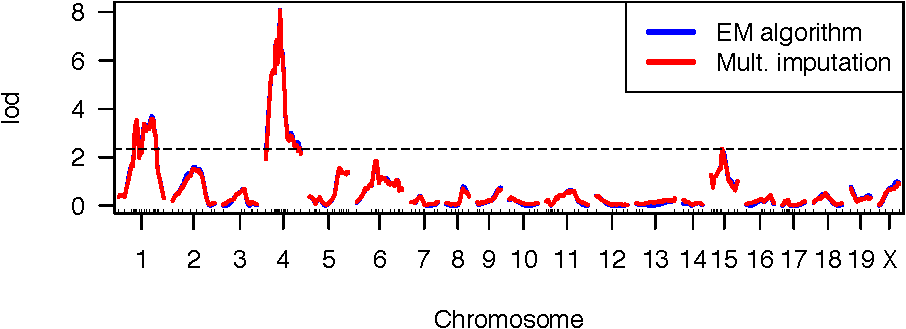
\includegraphics{_main_files/figure-latex/qtl-plot-out-1.pdf}
\caption{\label{fig:qtl-plot-out}QTL plot showing LOD scores and QTL
positions with EM algorithm and the multiple imputation. The dotted line
indicates the genome-wide LOD score threshold for a p \textless{} 0.05.
Every peak above this threshold is considered a QTL.}
\end{figure}

\paragraph{QTL interaction mapping}\label{qtl-interaction-mapping}

\paragraph{Covariates in QTL models}\label{covariates-in-qtl-models}

\subsubsection{\texorpdfstring{QTL Analysis using Bayesian Interval
Mapping (``qtlbim''
package)}{QTL Analysis using Bayesian Interval Mapping (qtlbim package)}}\label{qtl-analysis-using-bayesian-interval-mapping-qtlbim-package}

\section{Gene x Environment
interactions}\label{gene-x-environment-interactions}

\section{Variance and heritability}\label{variance-and-heritability}

\section*{Exercises: Quantitative
Genetics}\label{exercises-quantitative-genetics}


\chapter{Genetics of complex
diseases}\label{genetics-of-complex-diseases}

\section{Genome Wide Association Studies
(GWAS)}\label{genome-wide-association-studies-gwas}

\begin{itemize}
\tightlist
\item
  design and analysis of genetic association studies
\end{itemize}

\section{Pedigree analysis}\label{pedigree-analysis}

\chapter{Genetic Epidemiology}\label{genetic-epidemiology}

\section{Infection models}\label{infection-models}

\cleardoublepage 

\appendix \addcontentsline{toc}{chapter}{\appendixname}


\chapter{More to Say}\label{more-to-say}

Yeah! I have finished my book, but I have more to say about some topics.
Let me explain them in this appendix.

To know more about \textbf{bookdown}, see \url{https://bookdown.org}.

\bibliography{packages.bib,book.bib}

%\usepackage{makeidx}\makeindex
\printindex

\end{document}
